\newpage
\section{Auswertung}
  \subsection{Vermessung des Röntgenstrahls}
    Die Intensitäten aus dem Detektorscan werden zunächst gegen die zugehörigen Winkel aufgetragen. An diese, in Grafik \ref{fig:gauß} zu sehende, Verteilung wird eine Gauß-Kurve der Form

    \begin{equation*}
      f(\alpha) = \frac{\text{A}}{\sqrt{2\pi}\sigma} \exp\left(-\frac{\left(\alpha - \alpha_0\right)^2}{2\sigma^2}\right)
    \end{equation*}
            
    mit den Parametern

    \begin{enumerate}
      \item $\sigma = \SI{0.0451}{\degree}$
      \item $\alpha_0 = \SI{-0.0014}{\degree}$
      \item $\text{A} = \SI{102336.14}{\degree}$
    \end{enumerate}

    angepasst.

    Aus der Standardabweichung $\sigma$ wird die volle Breite bei halbem Maximum

    \begin{equation*}
      \text{FWHM} = 2\sigma\sqrt{2\ln(2)} = \SI{0.1062}{\degree}
    \end{equation*}

    und aus der Standardabweichung sowie der Amplitude A die maximale Intensität des Röntgenstrahls

    \begin{equation*}
      I_0 = \si{905520.89}\,\frac{\text{Counts}}{\text{s}}
    \end{equation*}

    bestimmt.

    \FloatBarrier
    \begin{figure}[h]
        \centering
        \includegraphics[width = \textwidth]{gauß.pdf}
        \caption{Die beim Detektorscan gemessene Intensität ist gegen den Messwinkel aufgetragen, sodass sich die Halbwertsbreite des Strahls sowie dessen maximale Intensität über eine Gauß-Anpassung ermitteln lassen.}
        \label{fig:gauß}
      \end{figure}
  
    \FloatBarrier


  \subsection{Bestimmung des Geometriewinkels}
    Bei kleinen Einfallswinkeln trifft der Röntgenstrahl auch neben die Probe, sodass die maximal mögliche reflektierte Intensität abfällt. Dies soll für Winkel kleiner dem Geometriewinkel korrigiert werden.
    Dieser wird zunächst über den ersten Rockingscan bestimmt. Die dabei aufgenommene Intensität wird gegen den Einfallswinkeln $\alpha$ aufgetragen. Der Geometriewinkel $\alpha_{\text{g}}$ kann zu Beginn der
    ansteigenden Intensitätsflanke und am Ende der absteigenden Intensitätsflanke abgelesen werden. Der Mittelwert aus den abgelesenen und in Grafik \ref{fig:rockingscan} eingezeichneten Winkeln ergibt sich zu

    \begin{equation*}
      \overline{\alpha_{\text{g, grafisch}}} = \SI{0.64}{\degree}.
    \end{equation*}

    \FloatBarrier
    \begin{figure}[h]
        \centering
        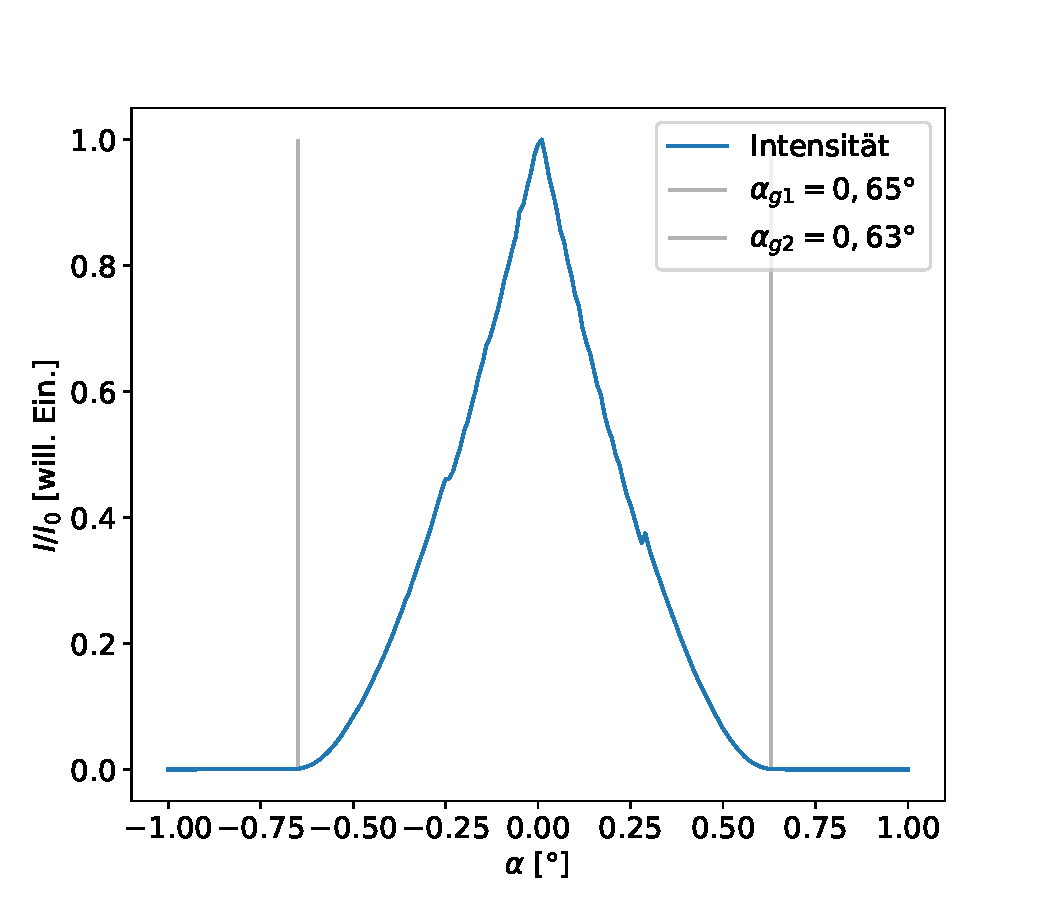
\includegraphics[width = \textwidth]{rockingscan_1.pdf}
        \caption{Die gemessene Intensität ist gegen den Winkel der Verdrehung der Probe relativ zum Strahl aufgetragen, sodass sich an dem Flankenanfang bzw. Flankenende der Geometriewinkel ablesen lässt.}
        \label{fig:rockingscan}
      \end{figure}
  
    \FloatBarrier

    Parallel kann der Winkel auch aus der Länge der Probe in y-Richtung $D=\SI{20}{\milli\metre}$ und des Strahldurchmesser $d_0=\SI{22}{\milli\metre}$ bestimmt werden. Dieser wird direkt aus dem ersten z-Scan 
    abgelesen, dessen gemessene Intensitäten gegen die z-Position in Grafik \ref{fig:zscan} aufgetragen sind. Über diese Methode ergibt sich der Geometriewinkel zu

    \begin{equation*}
      \alpha_{\text{g, math}} = \arcsin\left(\frac{d_0}{D}\right) = \SI{0.63}{\degree}.
    \end{equation*}

    \FloatBarrier
    \begin{figure}[h]
        \centering
        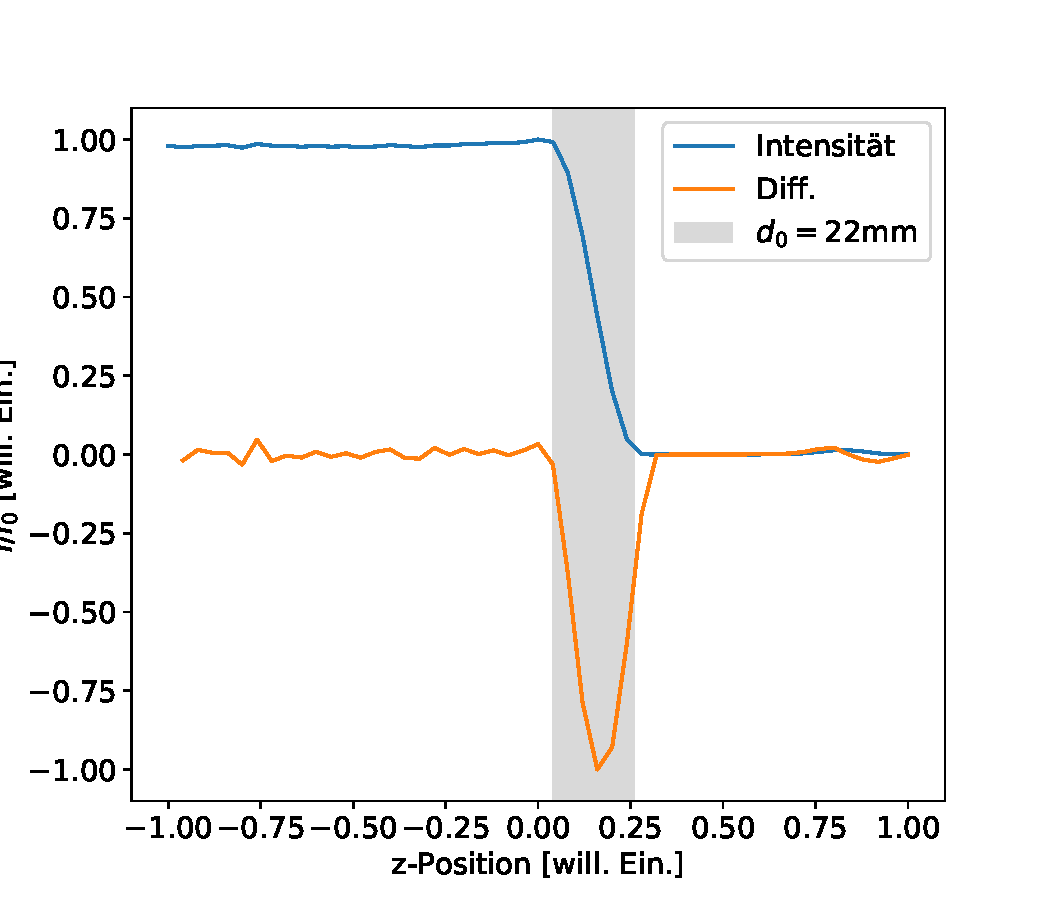
\includegraphics[width = \textwidth]{abschattung.pdf}
        \caption{Die Intensität ist gegen die z-Position der Probe aufgetragen. Zusätzlich ist auch die Ableitung dieses Verlaufs eingezeichnet, um die eingezeichnete Strahlbreite besser bestimmen zu können.}
        \label{fig:zscan}
      \end{figure}
  
    \FloatBarrier


  \subsection{Auswertungs des Reflektivitätsscans}
    Um die tatsächliche gemessene Reflektivität zu bestimmen, wird von der im Reflektivitätsscan gemessenen Intensität die Intensität, die durch diffuse Streuung entsteht, abgezogen und so eine tatsächliche 
    Reflektivität 
    
    \begin{equation*}
      R_{\text{exp}} = \frac{I_{\text{R}} - I_{\text{diffus}}}{I_0 \cdot 5}
    \end{equation*}
    
    bestimmt. Diese wird durch Normierung auf die fünffache maximale Intensität $I_0$ berechnet, da in der Messung zur Bestimmung der maximalen Intensität für \SI{1}{\second} und im Reflektivitätsscan für
    \SI{5}{\second} gemessen wurde. Die gemessene Reflektivität $R_{\text{exp}}$ und die über die Formeln \ref{eqn:R_F} und \ref{eqn:p} mit den Werten

    \begin{enumerate}
      \item $\lambda = \SI{1.54}{\angstrom}$
      \item $\alpha_{\text{c}} = \SI{0.223}{\degree}$
      \item $\mu = \SI{14100}{1\per\metre}$
    \end{enumerate}

    berechnete Fresnel-Reflektivität $R_{\text{F, Si, theo}}$ von Silizium sind in Grafik \ref{fig:Reflektivität_exp} eingezeichnet. Die Fresnel-Reflektivität $R_{\text{F, Si, theo}}$ ist wie zu erwarten für 
    Winkel kleiner dem kritischen Winkel gleich eins und fällt danach ab.

    \FloatBarrier
    \begin{figure}[h]
        \centering
        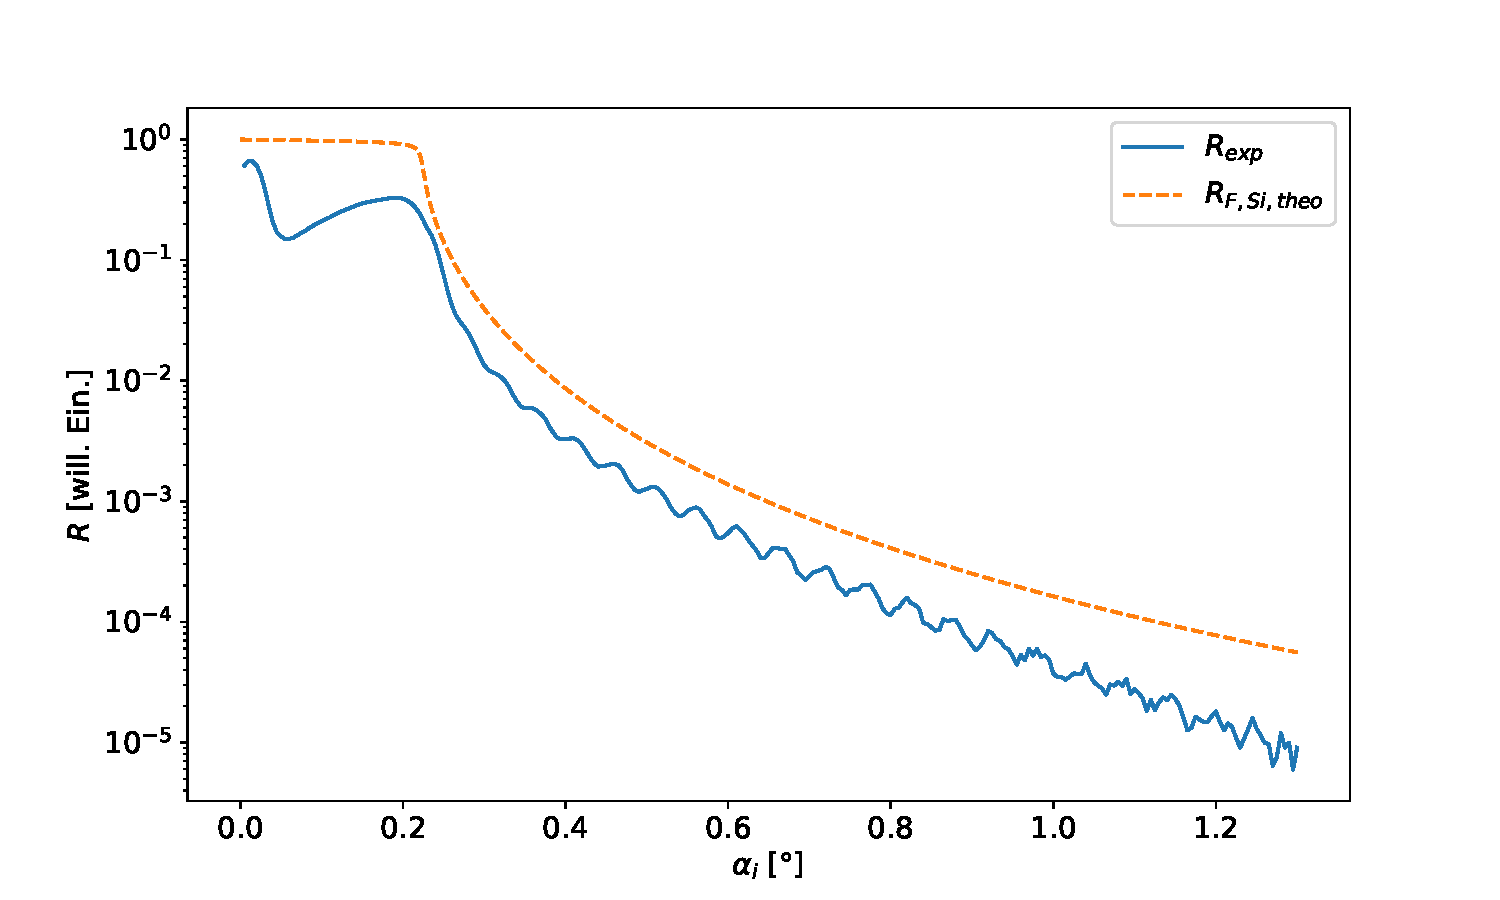
\includegraphics[width = \textwidth]{reflectivity_exp.pdf}
        \caption{Darstellung der gemessenen Reflektivität $R_{\text{exp}}$ sowie des theoretischen Verlaufs der Fresnel-Reflektivität für eine einzelne Siliziumoberfläche $R_{\text{F, Si, theo}}$.}
        \label{fig:Reflektivität_exp}
      \end{figure}
   
    \FloatBarrier

    Zur Bestimmung der Diffusion und der kritischen Winkel der beiden Materialien sowie der Schichtdicke des Polystyrols muss der Reflektivitätsscan detailliert ausgewertet werden. Dazu wir die gemessene 
    Reflektivität $R_{\text{exp}}$ durch den Geometriefaktor für Winkel kleiner dem Geometriewinkel korrigiert und so die korrigierte Reflektivität

    \begin{equation*}
      R_{\text{exp, cor}} = \frac{R_{\text{exp}}}{\text{G}} \qquad \text{mit} \qquad \text{G}=1 \quad \text{für} \quad \alpha_{\text{i}} \gtrsim \alpha_{\text{G}} \qquad \text{und} \qquad \text{G}=\frac{D\sin\left(\alpha_{\text{i}}\right)}{d_0} \quad \text{für} \quad \alpha_{\text{i}} < \alpha_{\text{G}}
    \end{equation*}

    berechnet. Die korrigierte Reflektivität $R_{\text{exp, cor}}$ ist in Abbildung \ref{fig:Reflektivität} dargestellt. 

    \FloatBarrier
    \begin{figure}[h]
        \centering
        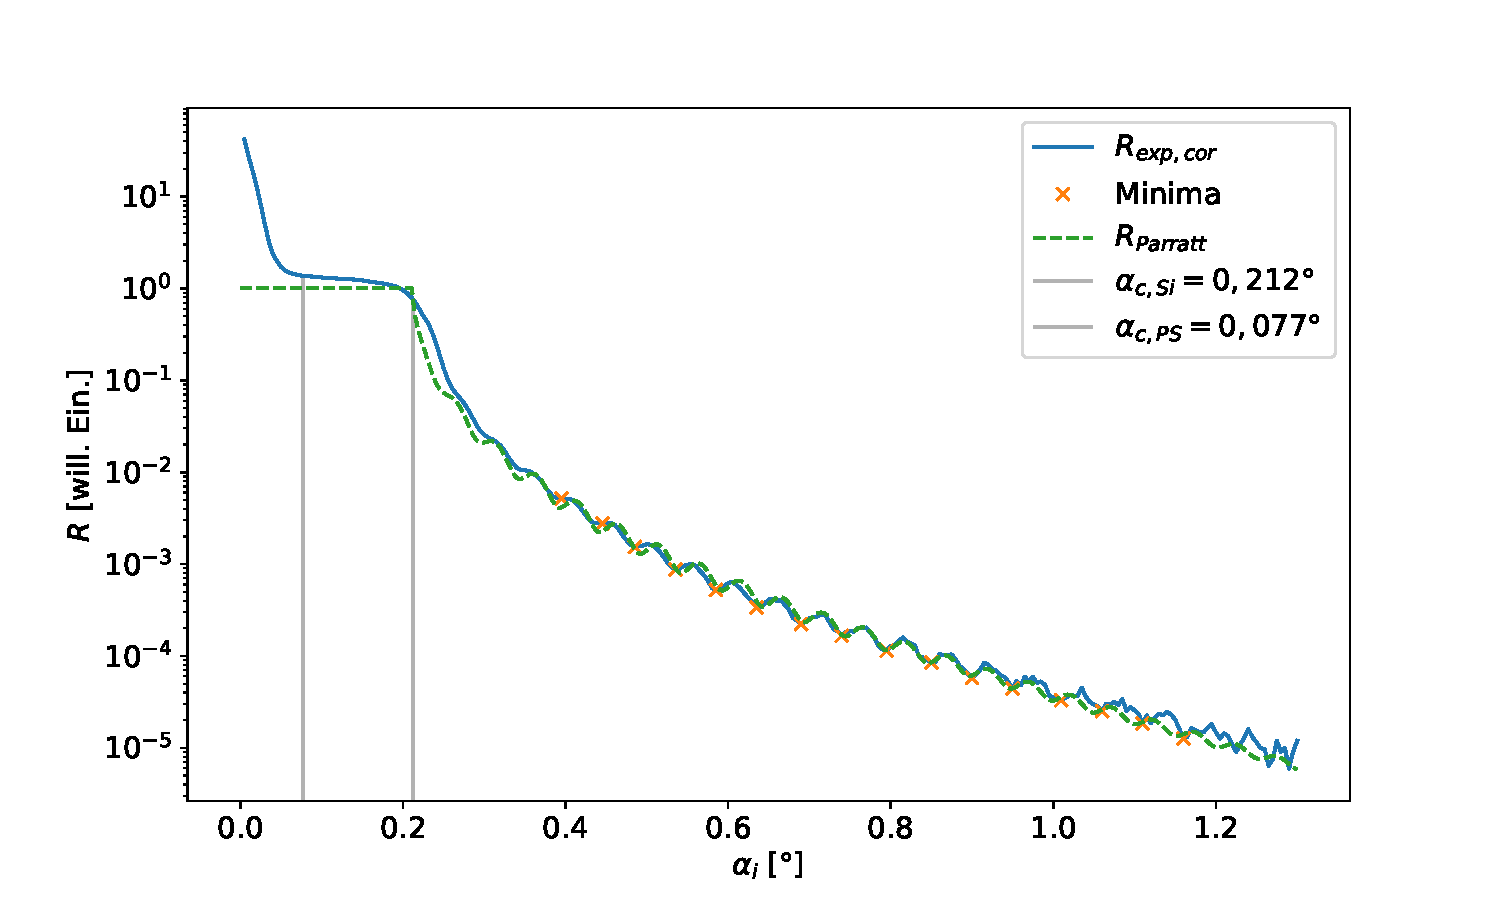
\includegraphics[width = \textwidth]{reflectivity_cor.pdf}
        \caption{Darstellung des durch den Korrekturfaktor G angepassten Verlaufs $R_{\text{exp, cor}}$ der gemessenen Reflektivität, an den die rekursiv über den Parratt-Algorithmus berechnete Reflektivität $R_{Parratt}$ angepasst wird. Aus dem Abstand der eingezeichneten Minima kann die Schichtdicke des Polystyrols bestimmt werden. Zusätzlich sind die kritischen Winkel für Silizium $\alpha_{\text{c, Si}}$ und Polystyrol $\alpha_{\text{c, PS}}$ eingezeichnet.}
        \label{fig:Reflektivität}
      \end{figure}
   
    \FloatBarrier

    Zur ersten Abschätzung der Schichtdicke werden die eindeutigen Minima der Kiessig-Oszillationen in der Kurve der korrigierten Reflektivität über das Python-Paket \textit{SciPy} ermittelt und der 
    mittlere Abstand dieser untereinander bestimmt:
    
    \begin{equation*}
      \overline{\Delta \alpha_{\text{i}}} = \SI{0.503+-0.011}{\degree}
    \end{equation*}
    
    Über Formel \ref{eqn:d_alpha} lässt sich die Schichtdicke $z_{\text{PS}}$ des Polystyrols so zu

    \begin{equation}
      z_{\text{PS}} = \SI{865+-19}{\angstrom}
      \label{eqn:z_ps}
    \end{equation}

    bestimmen.

    Anschließend wird die Reflektivität für ein System einer Polystyrol-Schicht auf einem Silizium-Substrat über den Parratt Algorithmus für raue Oberflächen simuliert.
    
    
    Die notwendigen Parameter der Polystyrol-Schichtdicke $z_2$, der Rauigkeit des Übergangs von Luft zu Polystyrol $\sigma_1$ und des Übergangs von Polystyrol zu Silizium $\sigma_2$ sowie der Dispersion von
    Polystyrol $\delta_2$ und Silizium $\delta_3$ werden händisch variiert, bis die rekursiv über die Formeln \ref{eqn:X_j}, \ref{eqn:k_z}, \ref{eqn:R_F_parratt} und \ref{eqn:r_rau} berechnete Reflektivität 
    bestmöglich mit der gemessenen übereinstimmt. Dazu wird 
    zunächst die Polystyrol-Schichtdicke auf den bereits berechneten Wert \ref{eqn:z_ps} gesetzt. Anschließend werden die Dispersionen angepasst, um die Kiessig-Oszillationen und die kritischen Winkel
    zu rekonstruieren. Abschließend werden die Rauigkeiten der Schichten angepasst, um den Verlauf der Einhüllenden für größere Winkel anzugleichen. Die in Abbildung \ref{fig:Reflektivität} dargestellte 
    Anpassung $R_{Parratt}$ wurde mit den folgenden Parameteren berechnet:
    
    \begin{enumerate}
      \item $z_2=\SI{866.0}{\angstrom}$
      \item $\sigma_1=\SI{1.080e-9}{1\per\angstrom}$
      \item $\sigma_2=\SI{7.056e-10}{1\per\angstrom}$
      \item $\delta_2=\SI{9.000e-7}{}$
      \item $\delta_3=\SI{6.840e-6}{}$
    \end{enumerate}

    Aus den Dispersionen werden die kritischen Winkel für Polystyrol und Silizium über

    \begin{equation*}
      \alpha_{\text{c}} = \sqrt{2\delta}
    \end{equation*}

    zu

    \begin{enumerate}
      \item $\alpha_{\text{c, PS}} = \SI{0.0769}{\degree}$
      \item $\alpha_{\text{c, Si}} = \SI{0.2119}{\degree}$
    \end{enumerate}
    
    bestimmt.